% A Beamer template for Central China Normal University 

\documentclass[aspectratio=169]{beamer}
\usepackage{ctex, hyperref}
\usepackage[T1]{fontenc}

% other packages
\usepackage{latexsym,amsmath,xcolor,multicol,booktabs,calligra}
\usepackage{graphicx,pstricks,listings,stackengine,subcaption}
\usepackage{CCNU}


\usefonttheme{serif}

\author{韩子坚}
\title{组会分享}    %标题
\subtitle{Case-Based or Rule-Based: How Do Transformers Do the Math? \\ Qwen2.5-Math Technical Report: Toward Mathematical Expert Model via Self-Improvement}    %副标题
\institute{华中师范大学计算机学院}    %机构
\date{\today}     %时间


% defs
\def\cmd#1{\texttt{\color{red}\footnotesize $\backslash$#1}}
\def\env#1{\texttt{\color{blue}\footnotesize #1}}
\definecolor{deepblue}{rgb}{0,0,0.5}
\definecolor{deepred}{rgb}{0.6,0,0}
\definecolor{deepgreen}{rgb}{0,0.5,0}
\definecolor{halfgray}{gray}{0.55}

\lstset{
    basicstyle=\ttfamily\small,
    keywordstyle=\bfseries\color{deepblue},
    emphstyle=\ttfamily\color{deepred},    % Custom highlighting style
    stringstyle=\color{deepgreen},
    numbers=left,
    numberstyle=\small\color{halfgray},
    rulesepcolor=\color{red!20!green!20!blue!20},
    frame=shadowbox,
}


\begin{document}

\kaishu %楷书

%homepage
\begin{frame}
    \titlepage
    % \begin{figure}[htpb]
    %     \begin{center}
    %         
\includegraphics[width=0.2\linewidth]{pic/CCNU.jpg}
    %     \end{center}
    % \end{figure}
\end{frame}

%content
\begin{frame}{Content}
    \tableofcontents[sectionstyle=show,subsectionstyle=show/shaded/hide,subsubsectionstyle=show/shaded/hide]
\end{frame}


\section{Case or Rule}
\subsection{case-based and rule-based 的原理}
\begin{frame}{case-based and rule-based 的原理}
    % \begin{itemize}[<+-| alert@+>] % 当然,除了alert,手动在里面插 \pause 也行
    %     \item 大家可能会\LaTeX{},不会的也会GPT,好多学校都有自己的Beamer主题
    %     \item 中文支持请选择 Xe\LaTeX{} 编译选项
    %     \item 原 THU Beamer 的项目地址位于 \url{https://github.com/tuna/THU-Beamer-Theme}
    %     \item 本项目地址位于 \url{https://github.com/Lanthanum1/CCNU-Beamer},如果有bug或者feature request可以去提issue
    % \end{itemize}
    \begin{columns}
        \begin{column}{0.2\textwidth}\onslide<2->{
            case-based 依赖训练时的语料库,如果语料库中没有需要推理的这个问题,则准确度会大幅下降。
        }
        \end{column}
            % \pause
        \begin{column}{0.6\textwidth} \onslide<1->{
    \begin{figure}[t]
        \centering        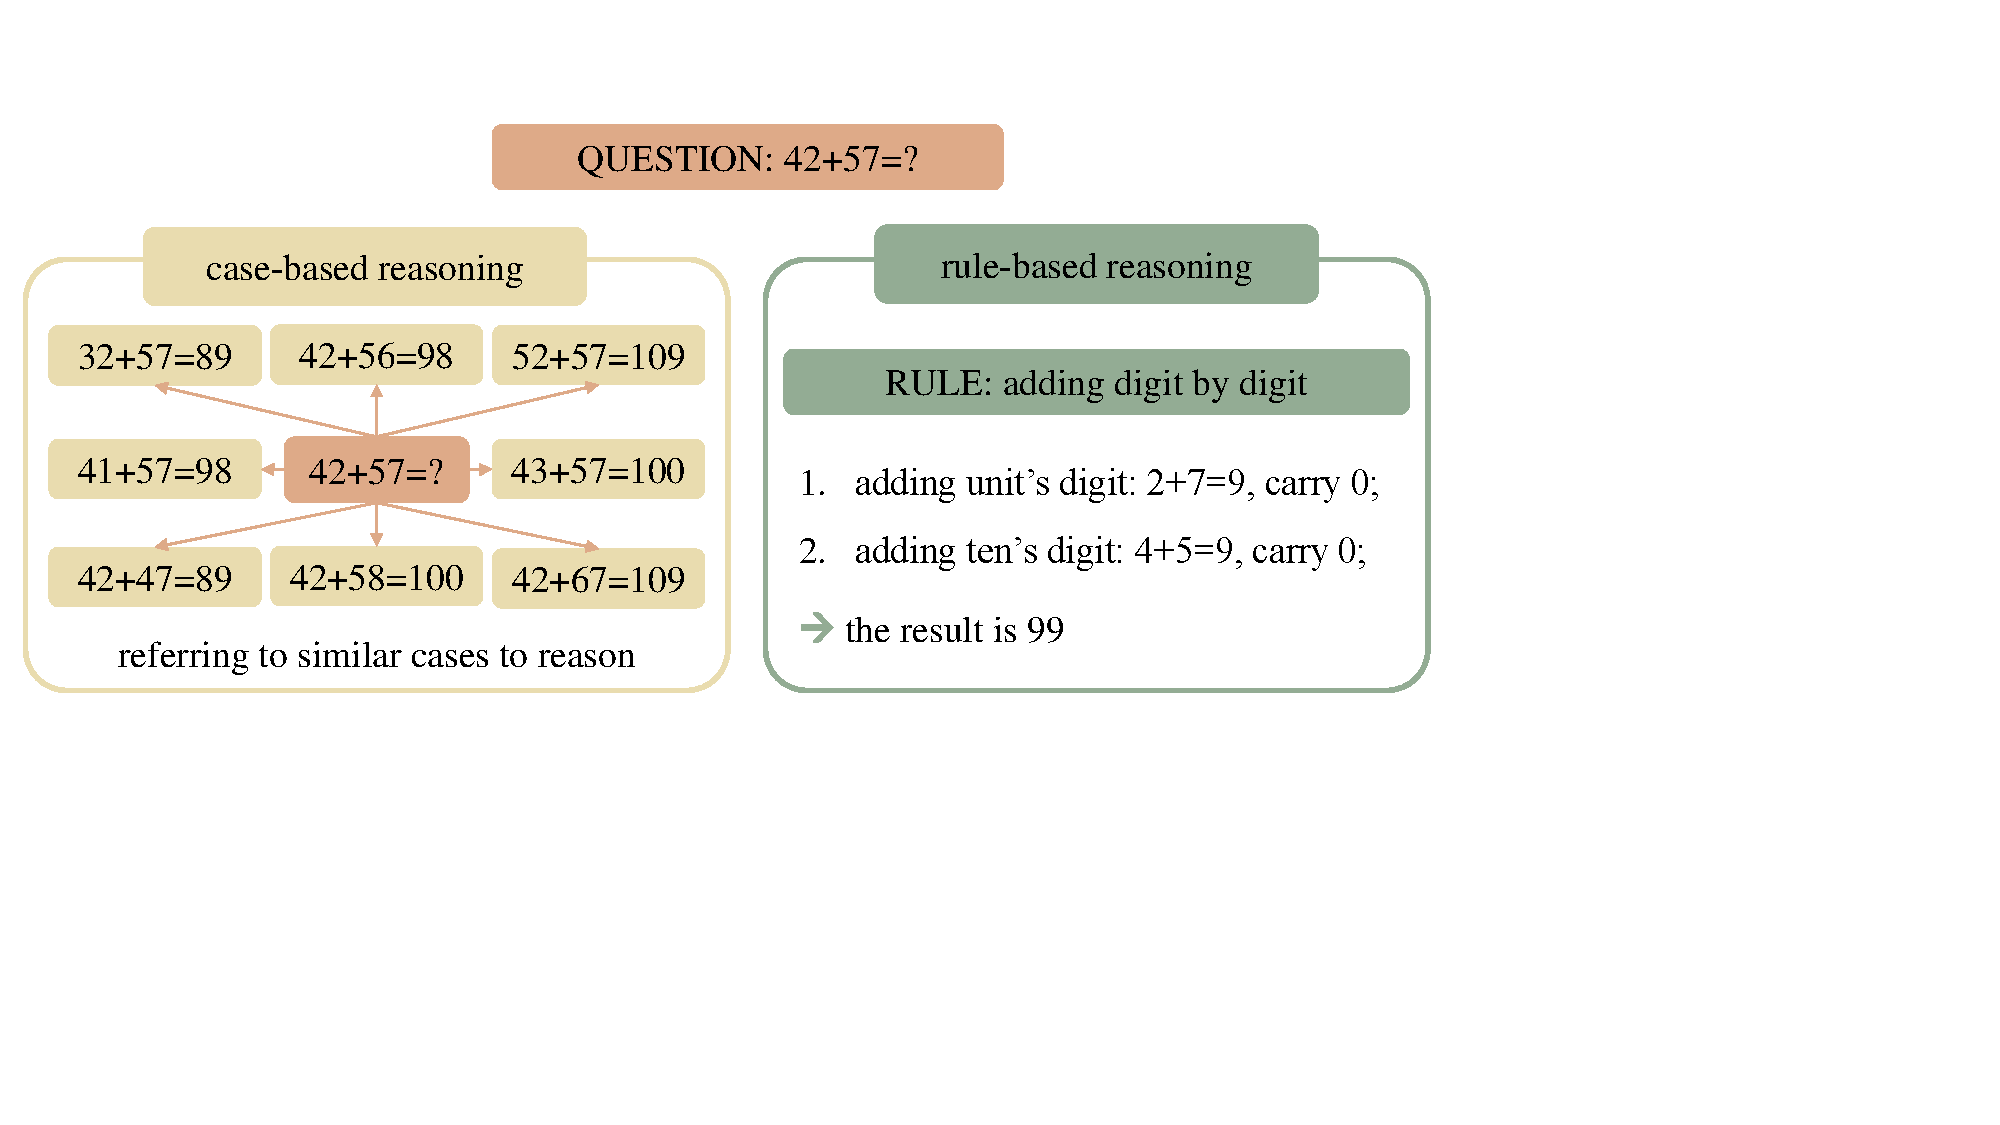
\includegraphics[width=\textwidth]{pic/case-or-rule.pdf}
        \caption{Illustrations of case-based and rule-based reasoning.}
        \label{case-or-rule}
    \end{figure}
        }
\end{column}
% \pause
\begin{column}{0.2\textwidth}\onslide<3->{
            rule-based 依赖数学规则,即使语料库中没有这个问题,也可以根据从语料库中学习到的数学规则推理出正确的答案。}
        \end{column}
    \end{columns}
\end{frame}

\subsection{Leave-Square-Out method}
\begin{frame}{Leave-Square-Out method} \small
    % \begin{exampleblock}{什么是Leave-Square-Out method?}
        Leave-Square-Out method (留方法,LSO) 是作者提出的一种交叉验证(cross-validation)方法,用于评估机器学习模型的性能。它是留一法(Leave-One-Out)的扩展。与留一法相比,Leave-Square-Out 方法不是每次只留一个样本进行测试,而是每次留出 $k^2$ 个样本进行测试,其中 $k$ 是一个正整数。当数据集规模较大时,这种方法可以更好地评估模型的泛化能力。
        \pause
    % \end{exampleblock}
    \begin{figure}[t]
        \centering
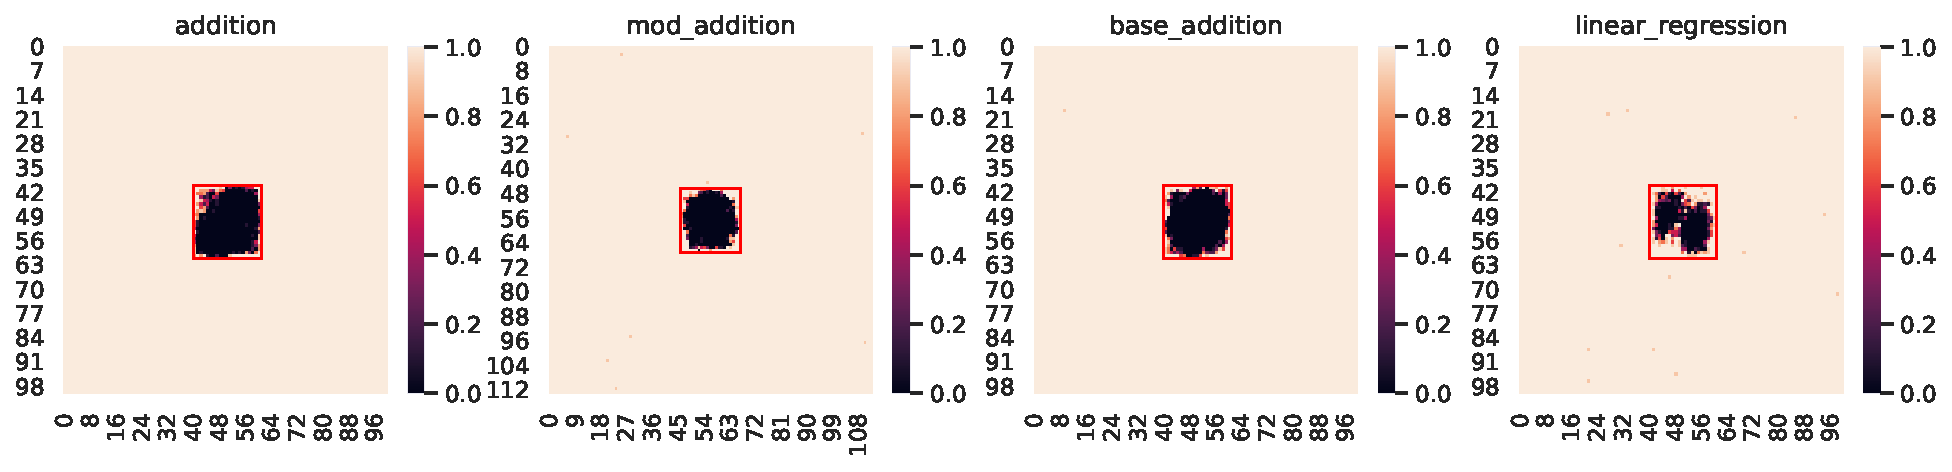
\includegraphics[height=0.3\textheight]{pic/1holes_w_rec_red_compressed.pdf}
        % \vspace{-10pt}
        \caption{Accuracy of Leave-Square-Out method}
        \label{fig:holes}
    \end{figure}
    \pause
    The appearance of holes in the figure indicates that the test samples away from the boundary of the training set are hard for the models to correctly infer.
\end{frame}

\subsection{rule-based setting}
\begin{frame}{rule-based setting} 
    \begin{exampleblock}{rule based 的重要性}
        Rule-based reasoning is essential for models to achieve systematic and length generalization so that they can be applied to new, unseen scenarios without re-training.
    \end{exampleblock}
\pause
    \begin{exampleblock}{rule based 应注意的事情}
        training set should always provide the necessities for the model to learn the underlying rule. For example, the training set should at least cover all the tokens used in the test set in order to develop a systematic rule that applies to the whole dataset.
    \end{exampleblock}
          
\end{frame}

\subsection{实验结论}
\begin{frame}{实验结论} 
    \begin{itemize}
        \item test squares 的位置不会影响实验结果
        \pause
        \item test squares 的大小会影响实验结果(the hole disappears when the test square shrinks to less than a small size)
        \pause
        \item scratchpad cannot teach transformers to perform rule-based reasoning. (why? scratchpad fine-tuning fails to teach transformers the actually applied "rule" behind each step. This is like teaching children addition only by showing them examples, without telling them the rationales behind each step.)
        \pause
        \item 模型和数据集的增大几乎不会影响实验结果,“holes”仍然存在
    \end{itemize}
\end{frame}

\section{RFFT(Rule-Following Fine-Tuning)}

\subsection{RFFT 的步骤}


\begin{frame}
    \begin{columns}
        \begin{column}{.7\textwidth}
    \begin{figure}[t]
        \centering
        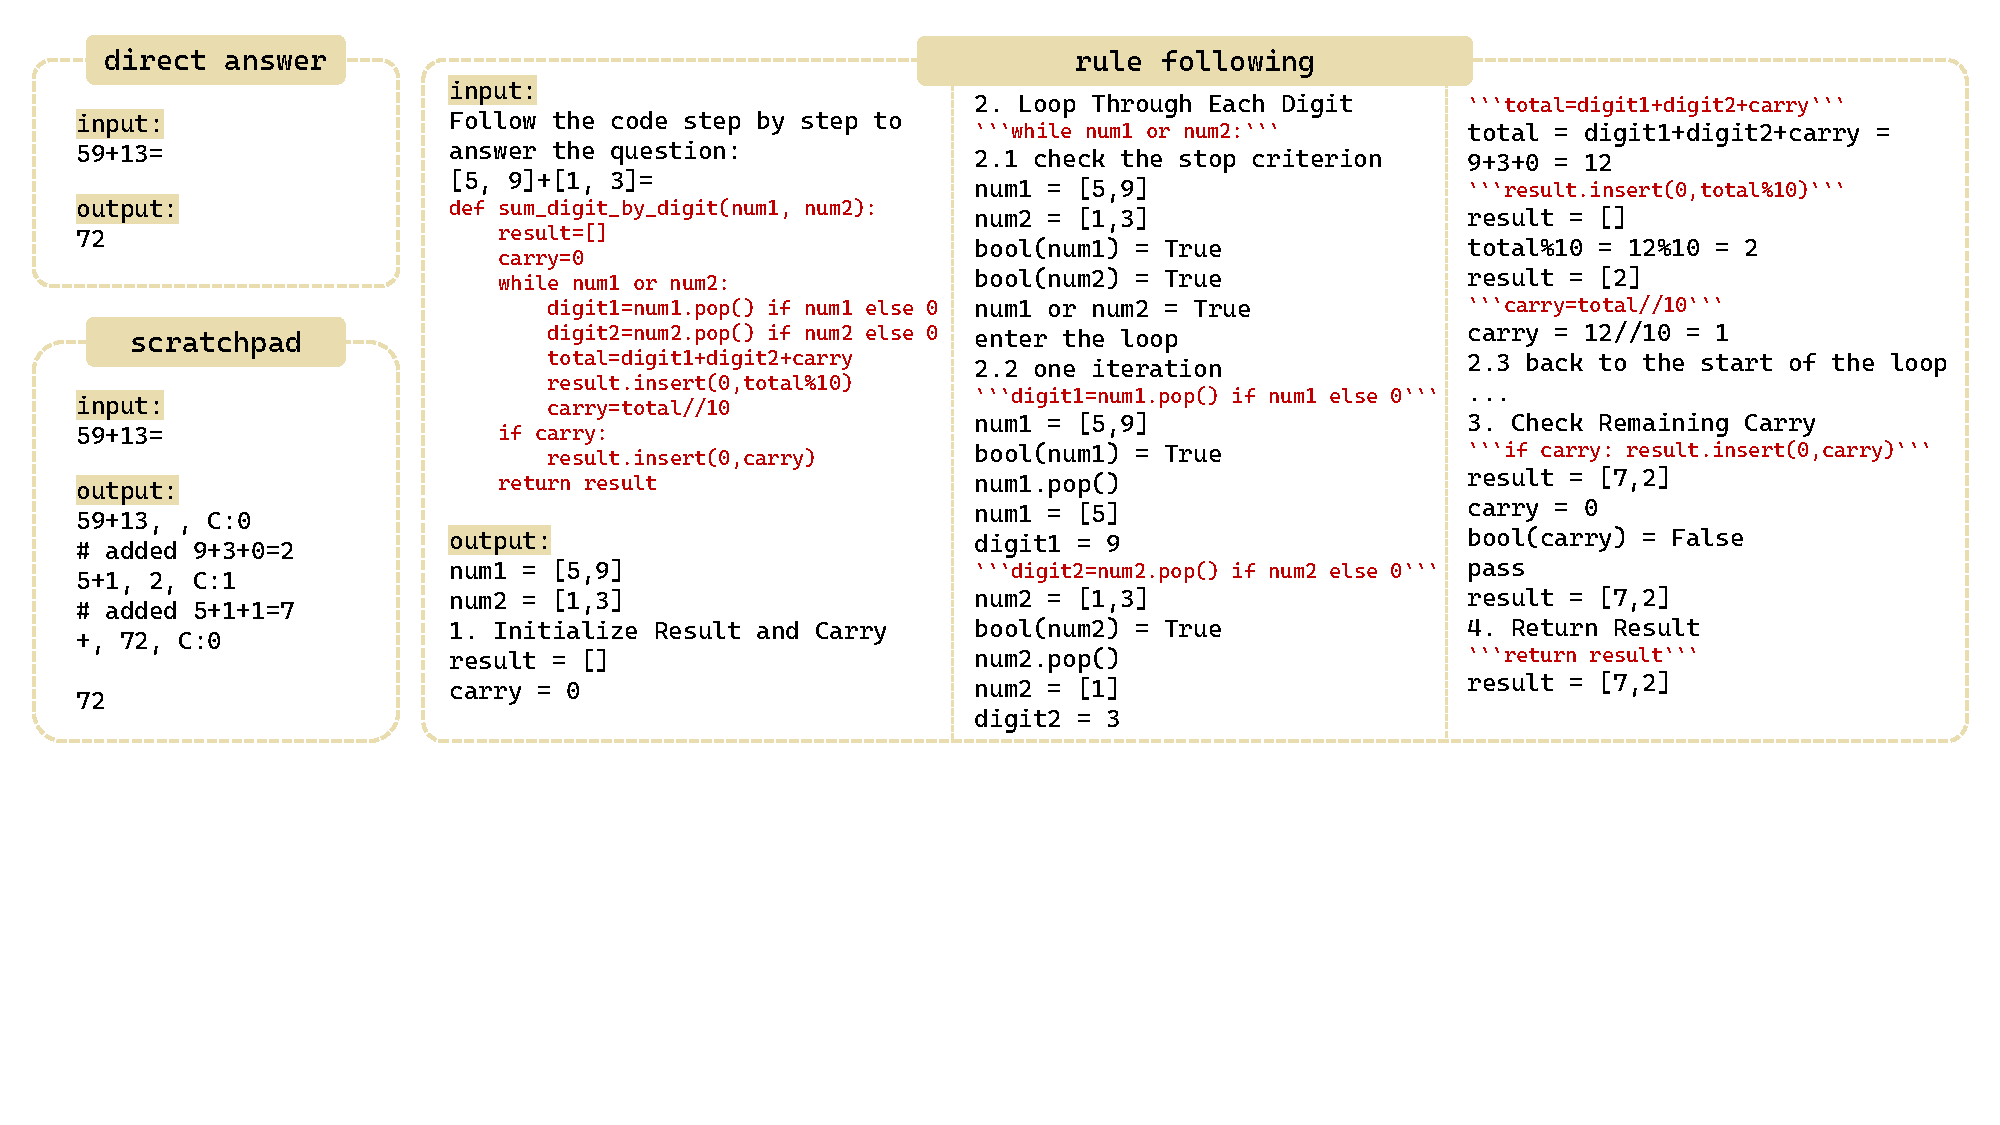
\includegraphics[width=\textwidth]{pic/prompt_new.pdf}
        \vspace{-5pt}
        \caption{Examples of input-output sequence of question $59+13$}
        \label{prompt}
    \end{figure}
\end{column}
\begin{column}{.3\textwidth}
    Step 1: Explicitly list the rules for solving a given task in the input.\\[0.2cm]

    Step 2: Finetune the model to follow the rules step by step.\\[0.2cm]

    可以有不用的方式阐述规则,including programs, pseudo-code, first-order logic, natural language, etc.
\end{column}
\end{columns}
\end{frame}

\subsection{RFFT 结果分析}
\begin{frame}{RFFT 结果分析} \begin{columns} \begin{column}{.7\textwidth} \begin{figure}[t] \centering \begin{subfigure}[t]{.45\textwidth} \centering 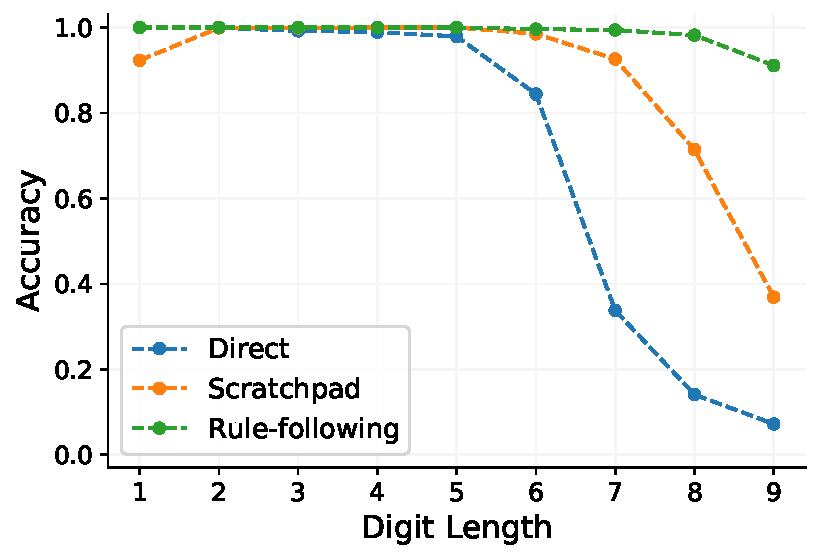
\includegraphics[width=\textwidth]{pic/llama_ft.pdf} \caption{Accuracy of Llama-7B fine-tuned with three methods tested on addition with 1-9 digits.} \label{fig:llama_ft} \end{subfigure}
    \hfill
    \begin{subfigure}[t]{.45\textwidth} \centering 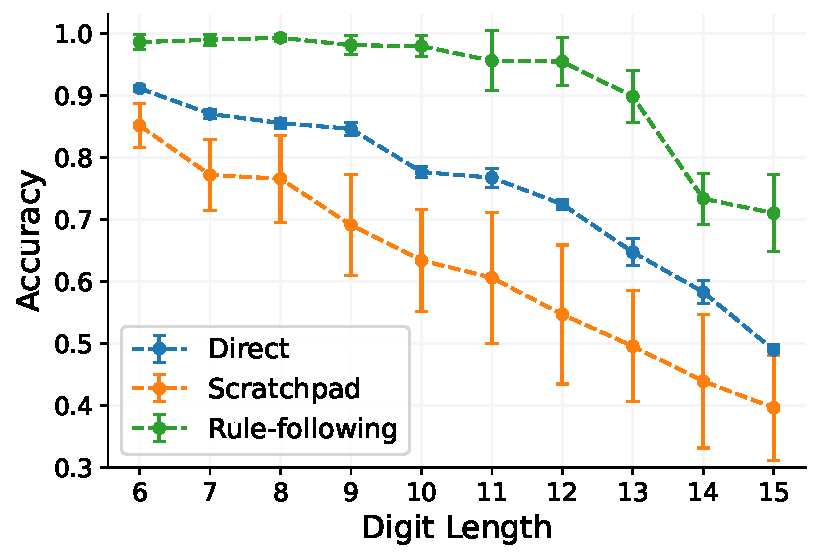
\includegraphics[width=\textwidth]{pic/gpt3_ft.pdf} \caption{Accuracy of GPT-3.5 fine-tuned with three methods tested on addition with 6-15 digits.} \label{fig:gpt3_ft} \end{subfigure}
    \caption{Accuracy of Llama-2-7B and GPT-3.5-turbo fine-tuned with direct answer, scratchpad and rule following on addition.}
    \label{fig:rfft} 
    \vspace{-5pt}
\end{figure}
\end{column}
\begin{column}{.3\textwidth} Llama-2-7B: RFFT: 91.1\% acc with 9-digit sums\\[0.2cm] scratchpad: less than 40\% acc\\[0.2cm] GPT-3.5-turbo: over 95\% acc on 12-digit addition (only 100 training samples) \end{column}
\end{columns}
\end{frame}

\subsection{误差分析}
\begin{frame}{误差分析}
    \begin{itemize}
\item RFFT 并不能带来100\%的准确性,作者发现大模型在计算时的每一步总能找到正确的规则,但是在一些基本的运算中会出现失误的现象,这可能是由于大模型幻觉或者是大模型处理长文本的局限性。\\[0.4cm]
\pause
\item RFFT as a Meta Learning Ability:stronger models indeed need less examples to learn rules.\\[0.4cm]
\pause
\item Given detailed rules, LLMs have certain abilities to follow the rules, which allows the models to show some reasoning ability on unfamiliar tasks. However, they do not gain a competitive edge from the rules in tasks already familiar to them.
    \end{itemize}
\end{frame}

            



\section{Qwen-2.5-Math}

\subsection{横向对比其他模型的得分表现}

\begin{frame}{横向对比其他模型的得分表现}
    \begin{figure}[htbp]
        \centering
        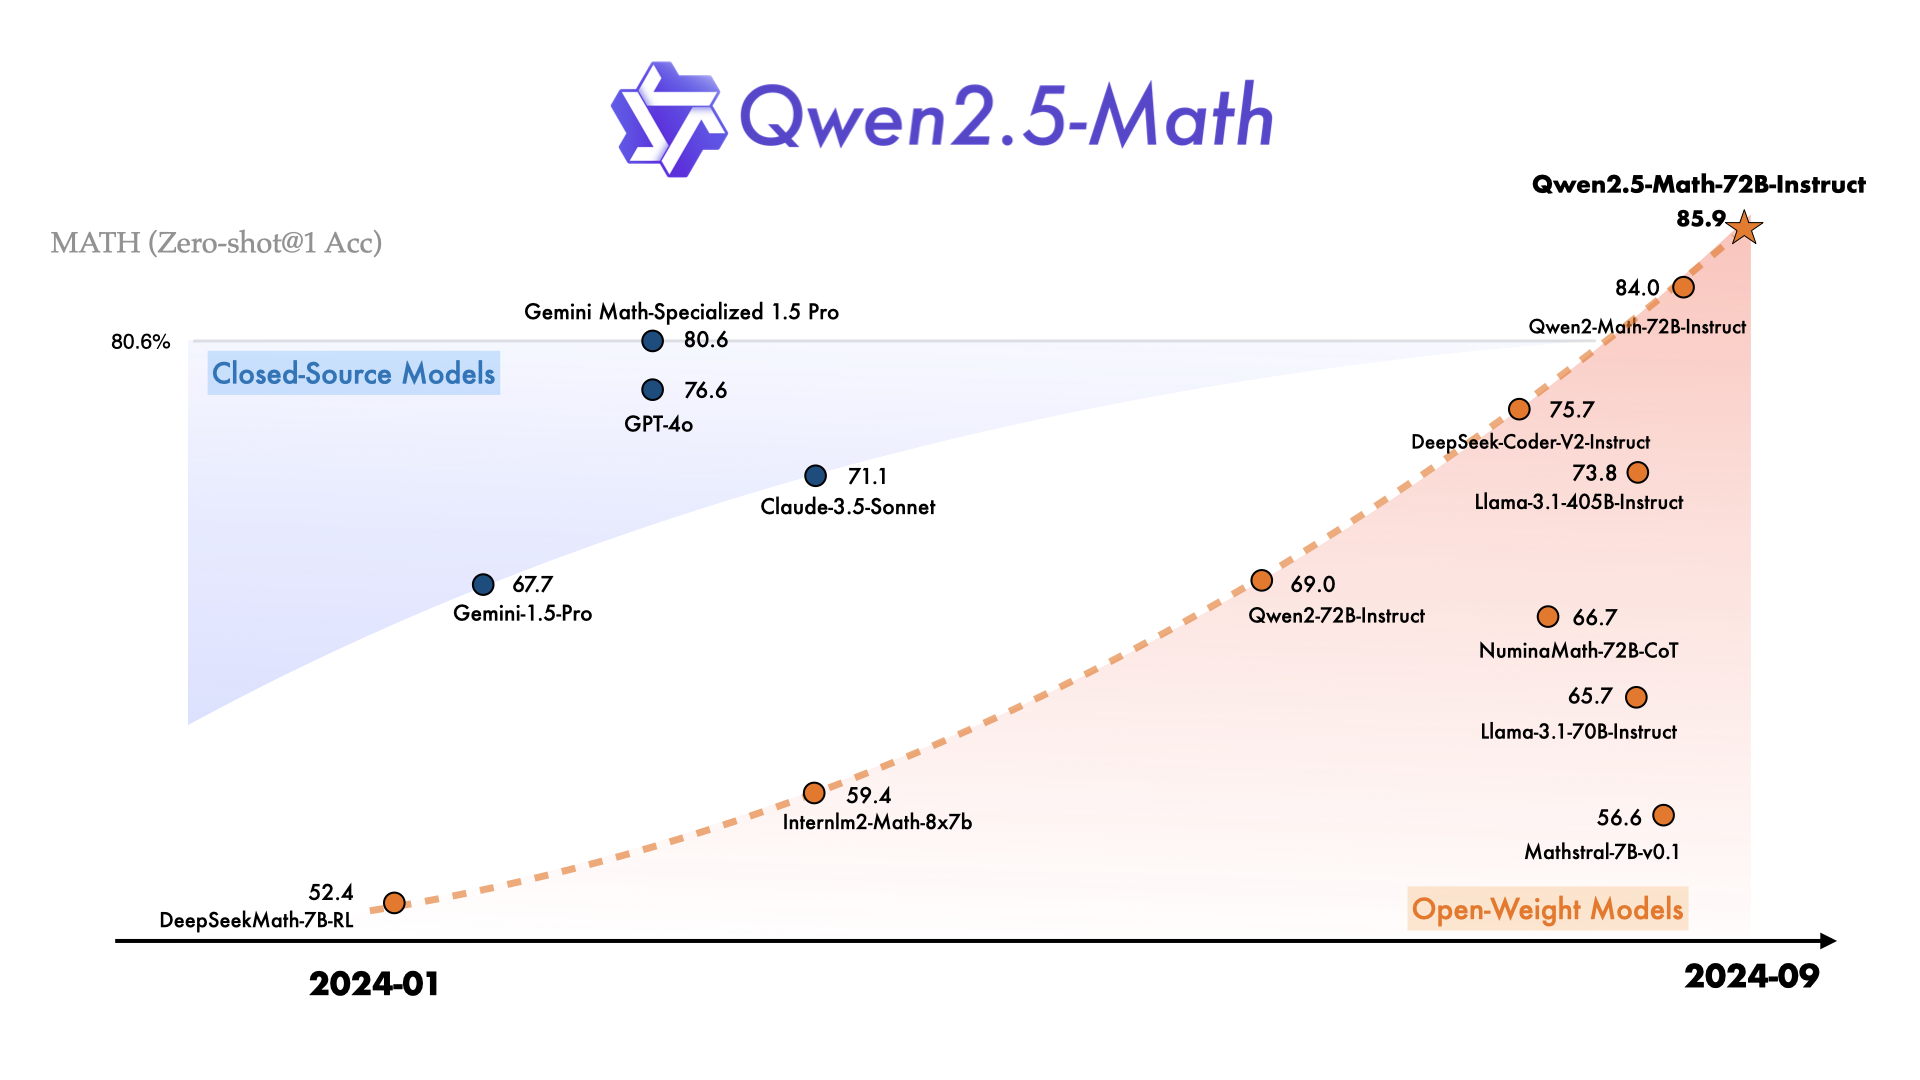
\includegraphics[width=0.7\textwidth]{pic/flagship.png}
        % \vspace{-1mm}
        \caption{The pass@1 performance of Qwen2.5-Math-72B-Instruct on MATH by the Chain-of-Thought reasoning.}
        \label{fig:intro}
    \end{figure}
\end{frame}

\subsection{Self-improvement techniques}
\begin{frame}{Self-improvement techniques}
    \begin{itemize}
        \item In pre-training, we employ Qwen2-Math-Instruct to synthesize math queries and corresponding responses on a large scale to enrich the pre-training corpus of Qwen2.5-Math.\\[0.2cm]
        \pause
        \item In post-training, we train a reward model on massive sampling from previous models and apply it to the iterative evolution of data in supervised fine-tuning.\\[0.2cm]
        \pause
        \item Use Qwen2.5-Math-RM in reinforcement learning and best-of-N sampling during inference.
    \end{itemize}

\end{frame}

\subsection{Qwen 2.5 math 的训练流程}
\begin{frame}{Qwen 2.5 math 的训练流程}\small
\begin{columns}
    \begin{column}{0.6\textwidth}
        \begin{figure}[htbp]
            \centering
        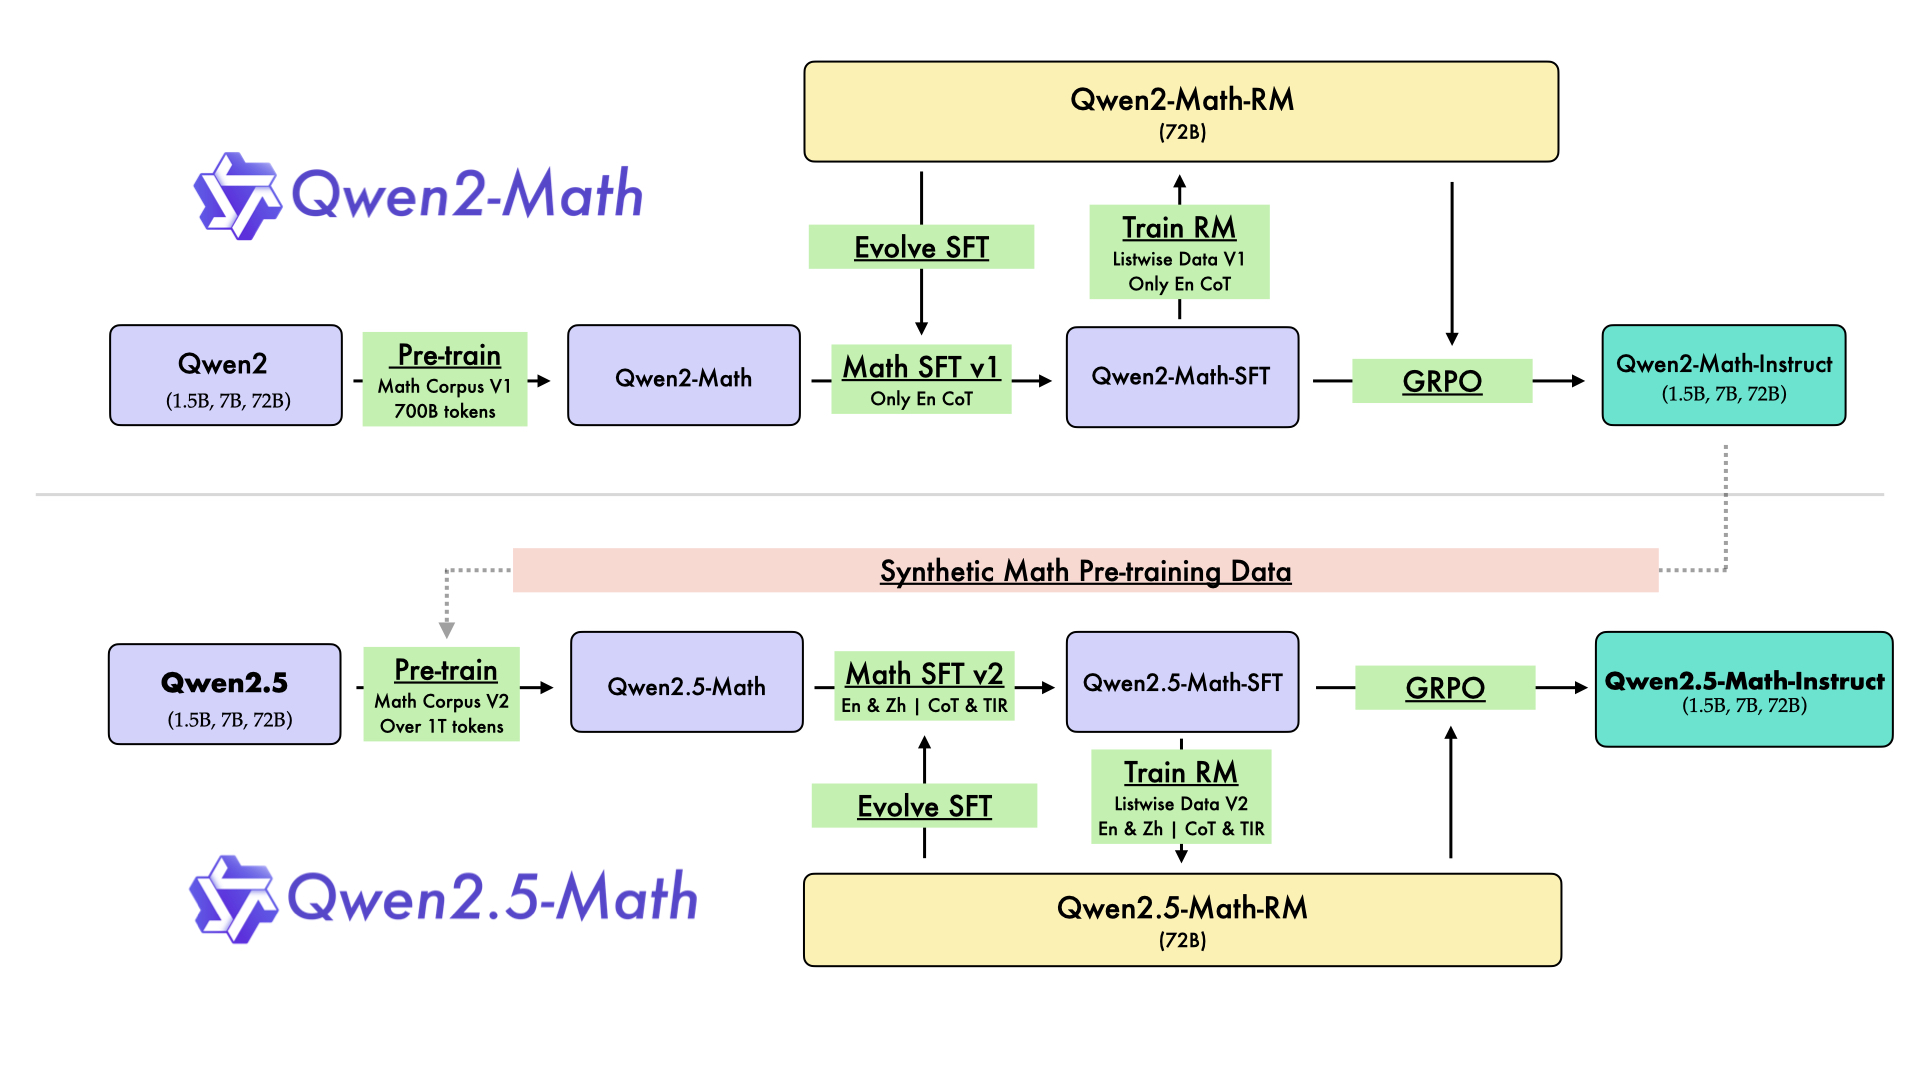
\includegraphics[width=1\columnwidth]{pic/qwen2.5-math-pipeline.jpeg}
            \vspace{-1mm}
            \caption{The development pipelines of Qwen2-Math and Qwen2.5-Math. }
            \label{fig:pipeline}
        \end{figure}
    \end{column}

    \begin{column}{0.4\textwidth}
        \begin{enumerate}
            \item Start -> Qwen Math Corpus v1 (700B tokens) -> Qwen2-Math Base Models
            \item Qwen2-Math-72B -> Qwen2-Math-RM -> SFT Data -> Qwen2-Math-Instruct
            \item Qwen2-Math-72B-Instruct -> Additional Data -> Qwen Math Corpus v2 (1T tokens)
            \item Qwen Math Corpus v2 -> Qwen2.5-Math Models
            \item Qwen2.5-Math-RM -> Qwen2.5-Math-Instruct
        \end{enumerate}
    \end{column}
\end{columns}
\end{frame}

\subsection{pre-training}
\begin{frame}{data}
    quantity:
    \begin{enumerate}
    \item Train a FastText classifier utilizing high-quality mathematical seed data and general text data.
\pause
    \item Leverage meta-information from the recalled data to expand the data pool for mathematical data retrieval.
    \pause
    \end{enumerate}
quality: 
\begin{enumerate}
    \item Utilize the Qwen2-0.5B-Instruct model, augmented with prompt engineering, to evaluate the quality of potential data entries.
    \pause
    \item Employ the Qwen2-72B-Instruct model to synthesize a large amount of mathematical pre-training corpus.
\end{enumerate}
\end{frame}

\subsection{post-training}
\begin{frame}{post-training}
    \begin{itemize}
        \item Aggregate more high-quality mathematical data, especially in Chinese, sourced from web documents, books, and code repositories across multiple recall cycles. Qwen Math Corpus v1(700B tokens) -- >Qwen Math Corpus v2(over 1T tokens)\\[.2cm]
        \pause
        \item Leverage the Qwen2.5 series base models for parameter initialization instead of initializing from the Qwen2 series.
    \end{itemize}


\end{frame}

\subsection{CoT and TIR}
\begin{frame}{CoT and TIR}
    \begin{exampleblock}{Chain-of-Thought Dataset Synthesis}
        \begin{itemize}
            \item Content: Comprises 580K English and 500K Chinese mathematical problems, collected from sources like GSM8K, MATH, and NuminaMath, and enriched with K-12 Chinese problems to enhance the Qwen2.5-Math model.
            \pause
\item Problem Complexity: A \textbf{difficulty-scoring model} is used to ensure a balanced distribution of problem complexities.
\pause
\item Response Construction: Utilizes iterative approaches with rejection sampling and reward modeling to refine responses, incorporating majority voting for synthesized problems without definitive answers. An additional refinement iteration is conducted for Qwen2.5-Math.
        \end{itemize}    
    \end{exampleblock}
\end{frame}

\begin{frame}{CoT and TIR}
    \begin{exampleblock}{Tool-Integrated Reasoning Data Synthesis}
        \begin{itemize}
            \item Objective: To overcome CoT prompting challenges related to computational accuracy and complex algebraic problem-solving by integrating a Python interpreter as a reasoning aid.
            \pause
            \item Dataset Content: Contains 190K annotated and 205K synthesized problems from datasets like GSM8K, MATH, and CollegeMath. An additional 75K problems are translated into Chinese to bolster proficiency in the language.
            \pause
            \item Response Construction: Employs online \textbf{Rejection Fine-Tuning (RFT)} to generate reasoning paths that align with reference answers. Nucleus sampling, deduplication, and majority voting techniques are used to ensure a diverse and accurate dataset for model fine-tuning.
        \end{itemize}
    \end{exampleblock}
\end{frame}

\subsection{实验结果}
\begin{frame}
    \begin{figure}[htbp]
        \centering
        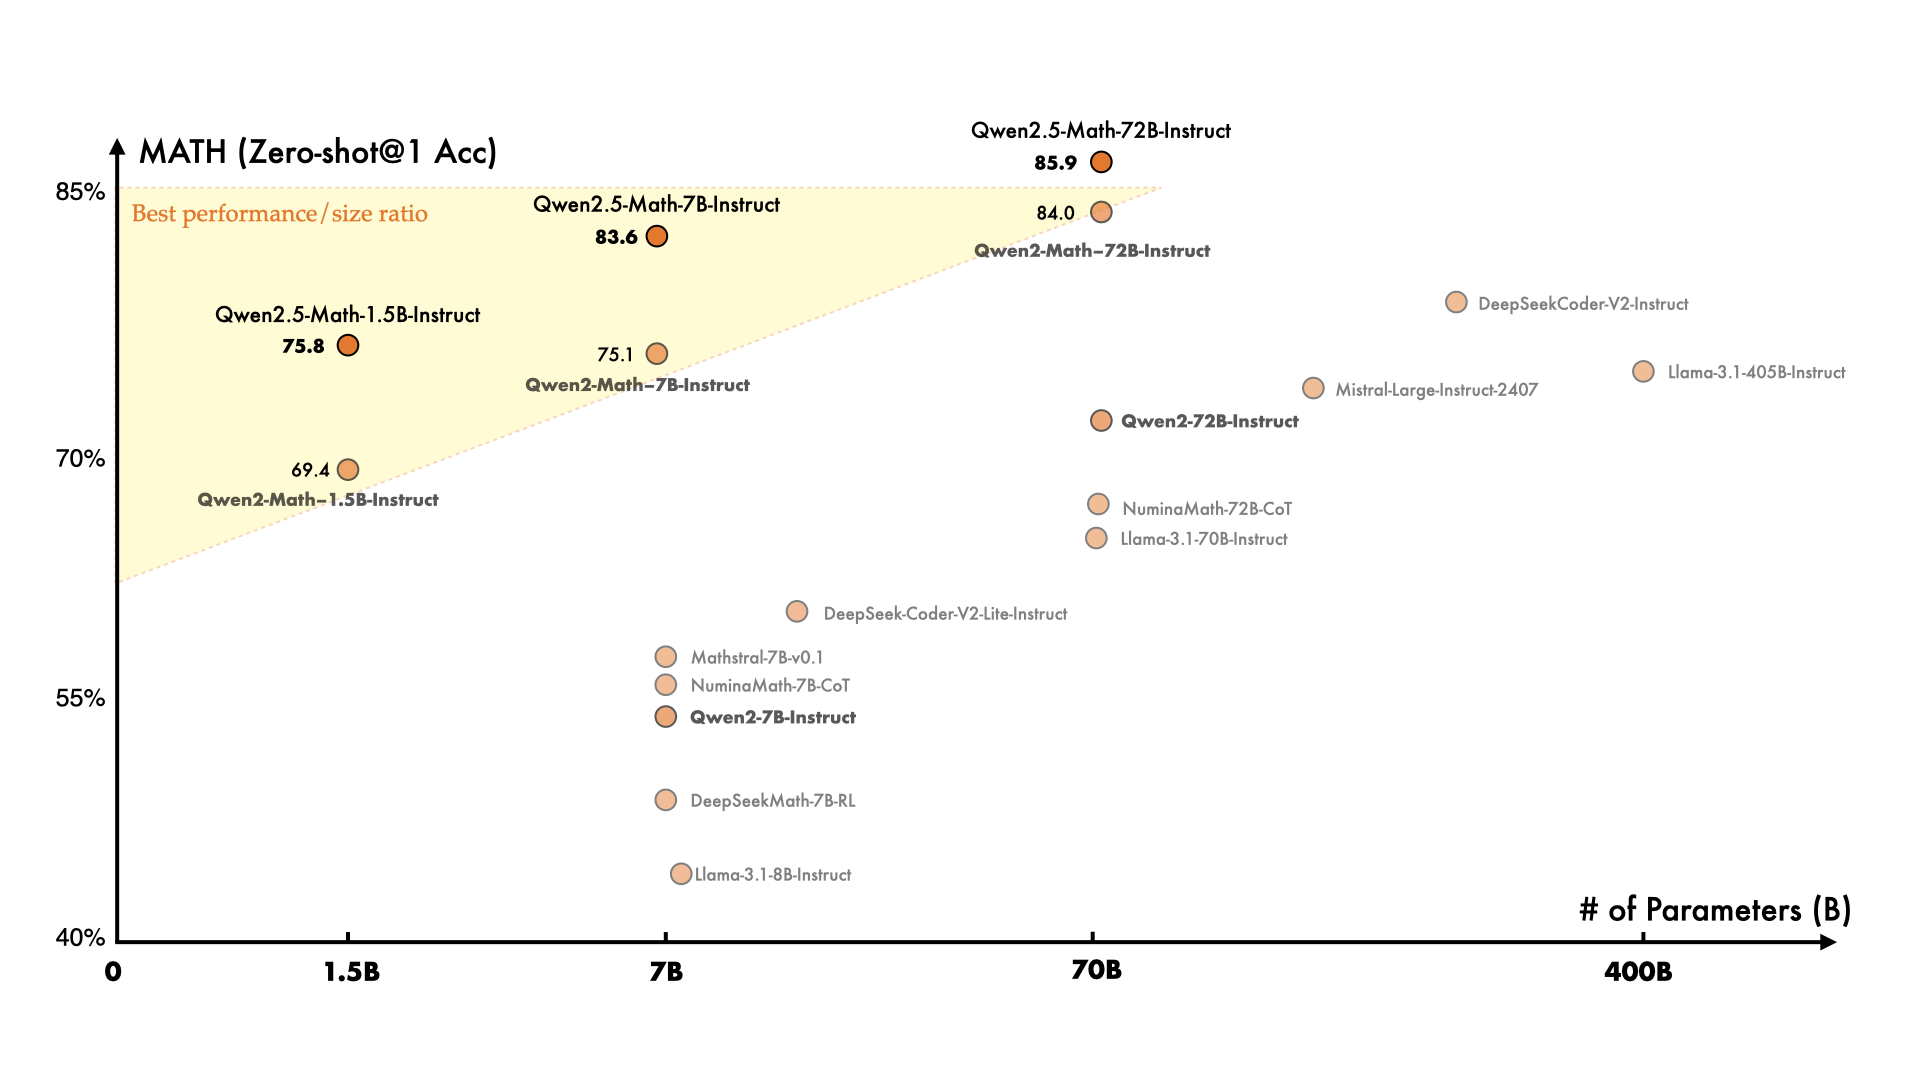
\includegraphics[width=0.8\columnwidth]{pic/all_size.png}
        \vspace{-1mm}
        \caption{The Performance of Qwen2.5-Math-1.5/7/72B-Instruct on MATH by CoT compared to models of the same size.}
        \label{fig:exp}
    \end{figure}
\end{frame}
    
\begin{frame}
    \begin{figure}[htbp]
        \centering
        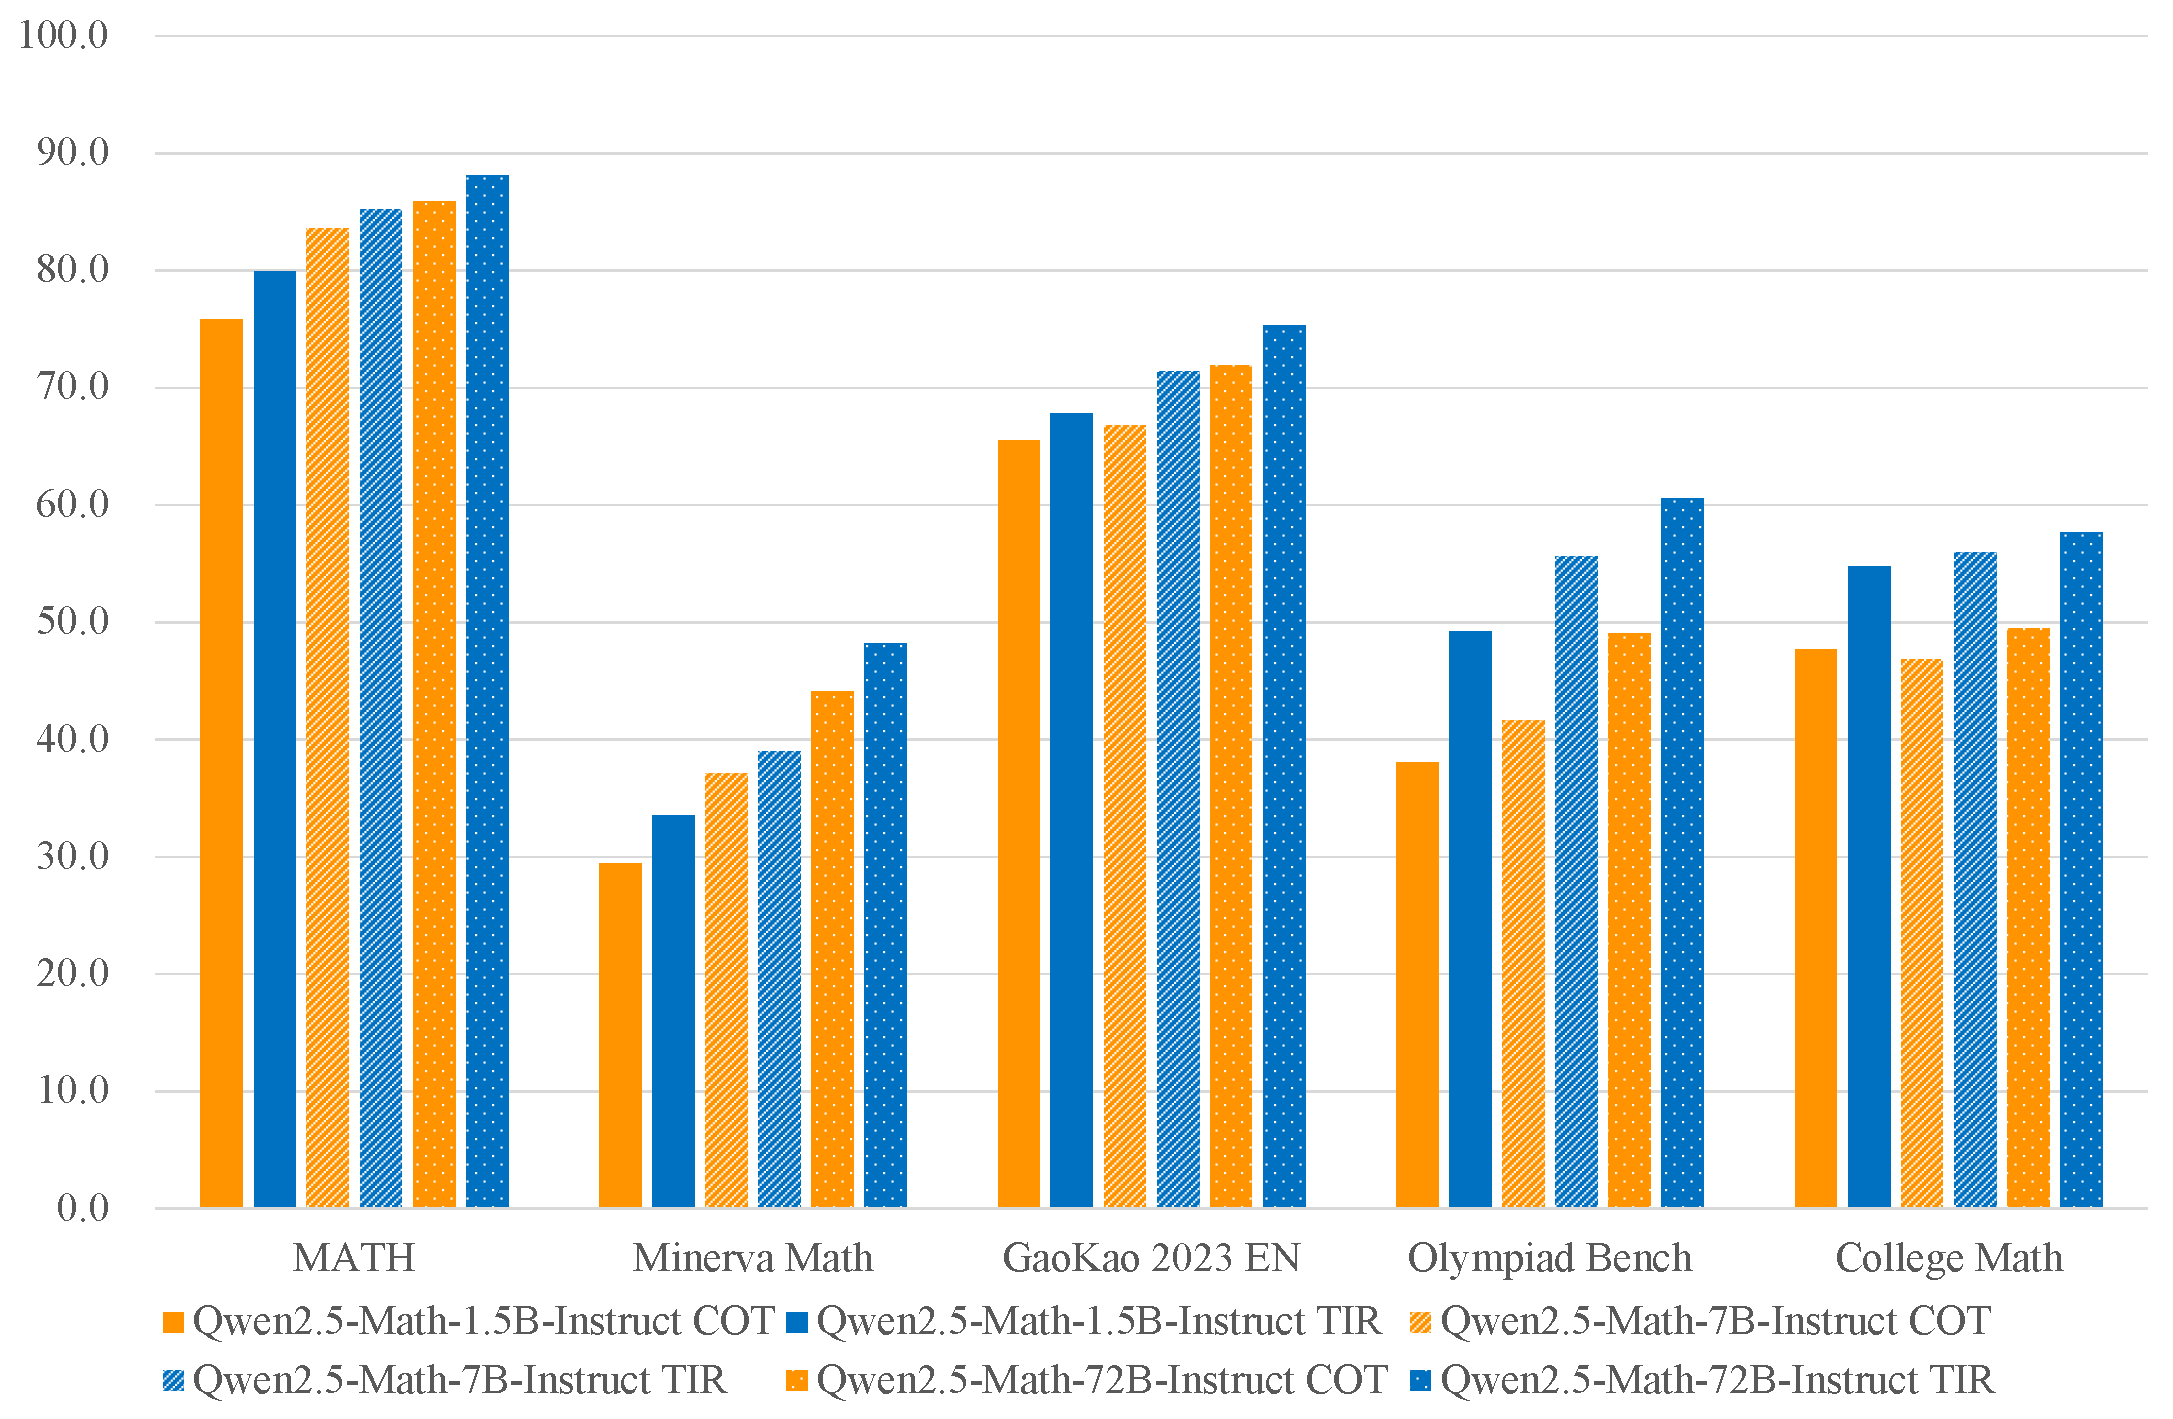
\includegraphics[width=0.7\columnwidth]{pic/COT_vs_TIR.pdf}
        % \vspace{-1mm}
        \caption{The Performance of Qwen2.5-Math-Instruct by using TIR compared to using CoT.}
        \label{fig:exp_tir}
    \end{figure}
\end{frame}





% \section{结束}

% \setbeamercolor{background canvas}{bg=ccnu}
% \begin{frame}[plain,t]
% \vspace{100pt}
% \centering
% 
\includegraphics[width=0.6\textwidth]{pic/hd_logo.jpg}
\begin{frame}
    \begin{center}
        {\Huge Thank you!}
    \end{center}
\end{frame}
% \end{frame}

\end{document}

